\scanpage{355}
$\mathcal L$
\deleted{$\underline{\operatorname{Hom}}($}
\[
\left\{\begin{aligned}
\underline{\operatorname{Hom}}_{\mathcal L}^!((\mathrm{Ss})^\circ,\mathcal B)&\simeq\underline{\operatorname{Hom}}_{\mathcal L}^!(\mathcal B_0,\mathcal B)\\
\underline{\operatorname{Hom}}_{\mathcal L}^!((\mathrm{Ss}),\mathcal A)&\simeq\underline{\operatorname{Hom}}_{\mathcal L}^!(\mathcal A_0,\mathcal A)
\end{aligned}\right.
\]
\diagram{\begin{tikzcd}
(\mathrm{Ss})^\circ\arrow[r,"F_0"] & \mathcal B_0\simeq(\mathrm{Ab}_*)^\circ\simeq(\mathrm{Ab}^{*})^\circ\\
(\mathrm{Ss})\arrow[r,no head,"G_0"] & \mathcal B
\end{tikzcd}}
\[
\left\{\begin{aligned}
\mathcal A_0&=\mathcal B_0^\circ,\quad\tikz[baseline=(bo.base)]{\node (bo) {$\mathcal B_0$};
\node[anchor=south] (ab) at ([yshift=7pt]bo.north) {$\simeq\mathrm{Ab}_*$};
\draw ([xshift=-7pt,yshift=-6pt]bo.west) .. controls ([xshift=-10pt,yshift=6pt]bo.west) and ([xshift=8pt,yshift=4pt]bo.north) .. (ab.east);}=\mathcal A_0^\circ\simeq(\mathrm{Ab}^*)^\circ\\
G_0&=(F_0)^\circ,\quad F_0=(G_0)^\circ
\end{aligned}\right.
\qquad F_0\in\mathrm{Ab}^{*}_{*}
\]
\[
\mathbb C_*\in
\]
\deleted{$\Omega_{\mathcal L}$}
\diagram{\left\{\begin{gathered}\begin{tikzcd}
\Omega_{\mathcal L}\simeq\mathcal B_0\arrow[r,hook',"\text{pl fid}"] & \mathrm{Ab}_*^\circ\simeq\mathrm{Ab}_\bullet^\circ\\
\Omega'_{\mathcal L}\simeq\mathcal A_0\arrow[r,hook',no head,"\text{pl fid}"'] & \mathrm{Ab}_*\simeq\mathrm{Ab}_\bullet
\end{tikzcd}\end{gathered}\right.}
\[
\underline{\operatorname{Hom}}(\Delta^\circ,\mathrm{Ab}_*^\circ)\simeq
\deleted{\underline{\operatorname{Hom}}(\Delta^\circ,}
(\mathrm{Ab}_*^*)^\circ
\]
\diagram{\begin{tikzcd}[column sep=small]
& & \unsure{\mathbb C^{*\alpha}|\mathbb C^{*\vee}}\arrow[dd,bend left=25]\\
& & \tikz[baseline=(z.base)]{\node(z){$\deleted{\unsure{\xi|\Delta}}$};\draw[rotate=15] (0,0) ellipse (.38 and .23);}\arrow[d]\\
\Omega\arrow[rr,bend left=25,no head]\arrow[rrr,bend left=30,no head] & F\arrow[r,no head]\arrow[rr,bend right=20,no head] & L_* & L_\bullet
\end{tikzcd}}
Cas $\mathcal A=\mathrm{Ab}$

op. contravariants de $\Omega$ dans $\mathrm{Ab}$
\figure{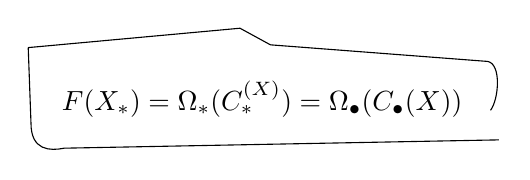
\begin{tikzpicture}
\node[inner sep=9pt] (fx) {$F(X_*)=\Omega_{*}(\mathbb C_*^{(X)})=\Omega_\bullet(\mathbb C_\bullet(X))$};
\draw ([xshift=-3pt,yshift=3pt]fx.north west) -- ([xshift=-8pt,yshift=10pt]fx.north)
 -- ([xshift=3pt,yshift=4pt]fx.north) -- ([yshift=-2pt]fx.north east)
 .. controls ([xshift=5pt,yshift=-3pt]fx.north east) and ([xshift=4pt]fx.east) .. ([xshift=1pt,yshift=-4pt]fx.east);
\draw ([xshift=-3pt,yshift=3pt]fx.north west) -- ([xshift=-2pt,yshift=7pt]fx.south west)
 .. controls ([xshift=-2pt,yshift=-3pt]fx.south west) and ([xshift=5pt,yshift=-3pt]fx.south west) .. ([xshift=10pt,yshift=-2pt]fx.south west)
 -- ([xshift=4pt,yshift=1pt]fx.south east);
\end{tikzpicture}}
\[
L_\bullet\quad L_*
\]
\[
\begin{aligned}
\operatorname{Hom}_{\widehat\Delta}(X_*,L_*)&\simeq\operatorname{Hom}_{*\to}(\mathbb C_*(X_*),L_*)\simeq\operatorname{Hom}_{\unsure{\mathrm{Ens}|\ge0}}(\mathbb C_\bullet(X),L_\bullet)\\
&\simeq\underline{\operatorname{Hom}}^*(\unsure{L^*_{\ge}|L^*_*},\mathbb C^*(X))\simeq\operatorname{Hom}^\bullet(L^\bullet,\mathbb C^\bullet(X))
\end{aligned}
\]
\margin{dans une\quad $L_*$ à augm.\quad Voy. adj.}

$\mathcal A\subset\widehat{\mathcal A}$
\[
\underline{\operatorname{Hom}}(\widehat\Delta_{\mathrm{ab}}\times\mathcal A^\circ,\mathrm{Ab})\simeq\underline{\operatorname{Hom}}(\mathcal A^\circ
\]
repr. p.r. aux deux arg.
\[
\varphi\in\underline{\operatorname{Hom}}_{!}(\underset{M}{\widehat\Delta_{\mathrm{ab}}},\underset{X}{\widehat{\mathcal A}})
\subset\underline{\operatorname{Hom}}(\widehat\Delta_{\mathrm{ab}}\times\mathcal A^\circ,\mathrm{Ab})
\]
\[
\operatorname{Hom}(X,\varphi(M))=\Phi(M,X)
\]
\margin{repr. en $X$
\figure{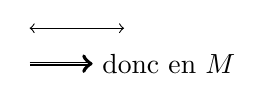
\begin{tikzpicture}
\draw[<->] (0,0)--(1.2,0);
\draw[double,->] (0,-.45)--(.8,-.45);
\node[right] at (.8,-.45) {donc en $M$};
\end{tikzpicture}}}
\deleted{$=\operatorname{Hom}(M,$}
\[
\Phi\operatorname{Hom}(\mathcal A^\circ,\underline{\operatorname{Hom}}_!,(
\]
\diagram{\begin{tikzcd}
\widehat\Delta\arrow[r,no head]&\mathrm{Ab}
\end{tikzcd}}
\diagram{\begin{tikzcd}
\underline{\operatorname{Hom}}_!(\widehat\Delta_{\mathrm{ab}},\mathcal A)\arrow[r]\arrow[dr] & \underline{\operatorname{Hom}}_!(\widehat\Delta,\mathcal A)\arrow[d,"\tikz[baseline=-.5ex]{\node[rotate=90]{$\simeq$};}"]\\
&\underline{\operatorname{Hom}}(\Delta,\mathcal A)\arrow[ul,bend left=30]
\end{tikzcd}}
\deleted{\[
X=\varinjlim_{\delta\in\Delta_{/X}}\delta
\]}
\diagram{\begin{tikzcd}[column sep=large]
\operatorname{Hom}(\varphi(X),M)=\Phi(X,M)\arrow[d,bend right=15]\arrow[dr] & : & \widehat\Delta_{\mathrm{ab}}^\circ\times\mathcal A\arrow[d]\\
\text{transf} & \text{repr. en }M & \mathrm{Ab}\\
\varinjlim\ \text{en}\\
\varprojlim\\
\text{donc repr. en }X
\end{tikzcd}}
\[
\simeq\operatorname{Hom}_{\widehat\Delta_{\mathrm{ab}}}(X,\psi(M))
\]
\diagram{\begin{tikzcd}
\widehat\Delta_{\mathrm{ab}}\arrow[r,shift left,"\varphi"] &\mathcal A\arrow[l,shift left,"\psi"]
\end{tikzcd}}
\diagram{\begin{tikzcd}
\mathcal A\arrow[r]&{}\\
\mathcal A\times\Delta\arrow[r,no head]&\mathrm{Ab}
\end{tikzcd}}
\mspage{356}
